% ****** Start of file apssamp.tex ******
%
%   This file is part of the APS files in the REVTeX 4.2 distribution.
%   Version 4.2a of REVTeX, December 2014
%
%   Copyright (c) 2014 The American Physical Society.
%
%   See the REVTeX 4 README file for restrictions and more information.
%
% TeX'ing this file requires that you have AMS-LaTeX 2.0 installed
% as well as the rest of the prerequisites for REVTeX 4.2
%
% See the REVTeX 4 README file
% It also requires running BibTeX. The commands are as follows:
%
%  1)  latex apssamp.tex
%  2)  bibtex apssamp
%  3)  latex apssamp.tex
%  4)  latex apssamp.tex
%
\documentclass[%
 reprint,
%superscriptaddress,
%groupedaddress,
%unsortedaddress,
%runinaddress,
%frontmatterverbose, 
%preprint,
%preprintnumbers,
%nofootinbib,
%nobibnotes,
%bibnotes,
 amsmath,amssymb,
 aps,
%pra,
%prb,
%rmp,
%prstab,
%prstper,
%floatfix,
]{revtex4-2}
\usepackage{kotex}
\usepackage{graphicx}% Include figure files
\usepackage{dcolumn}% Align table columns on decimal point
\usepackage{bm}% bold math
%\usepackage{hyperref}% add hypertext capabilities
%\usepackage[mathlines]{lineno}% Enable numbering of text and display math
%\linenumbers\relax % Commence numbering lines

%\usepackage[showframe,%Uncomment any one of the following lines to test 
%%scale=0.7, marginratio={1:1, 2:3}, ignoreall,% default settings
%%text={7in,10in},centering,
%%margin=1.5in,
%%total={6.5in,8.75in}, top=1.2in, left=0.9in, includefoot,
%%height=10in,a5paper,hmargin={3cm,0.8in},
%]{geometry}

\def\rcurs{{\mbox{$\resizebox{.16in}{.08in}{
\includegraphics{ScriptR}}$}}}
\def\brcurs{{\mbox{$\resizebox{.16in}{.08in}{
\includegraphics{BoldR}}$}}}
\def\hrcurs{{\mbox{$\hat \brcurs$}}}

\begin{document}


\title{전자 회절 실험 보고서}

\author{서울대학교 전기정보공학부 2018-12432 박정현}
 \email{alexist@snu.ac.kr}
\date{실험일자 : 09.25.2023}% It is always \today, today,
             %  but any date may be explicitly specified

\begin{abstract}
본 실험에서는 poly crystal 형태의 graphite를 투과한 전자의 회절 무늬를 측정하여 전자의 파동성을 확인하고 회절 격자 사이의 간격을 측정하였다. 기존에 알려진 graphite의 격자 간격값과 실험값이 적절한 재현도와 정확도에서 일치하였다. 본 실험에서 3차원 결정 구조를 파악할 수 없는 점, 그리고 다른 격자간격 값을 측정할 수 없음을 논하고 이를 수행할 수 있는 방법을 제시하였다.
\end{abstract}

%\keywords{Suggested keywords}%Use showkeys class option if keyword
                              %display desired
\maketitle

%\tableofcontents

\section{\label{sec:level1}Introudction}
\subsection{\label{sec:level2}Diffraction from Crystal}
주어진 결정 구조의 전자밀도 $n(\vec{r})$이 아래의 관계식을 만족한다고 가정하자. 이 때 $\vec{G}$는 reciprocal vector, $\vec{T}$는 translation vecotr로 각각 아래의 식을 만족한다.
\begin{align}
	n(\vec{r}+\vec{T}) &= \sum n_{G}\exp(i\vec{G}\cdot \vec{r})\exp(i\vec{G}\cdot\vec{T})
\end{align}
\begin{align}
	\vec{G} &= v_{1}\vec{b}_{1} + v_{2}\vec{b}_{2} + v_{3}\vec{b}_{3}\\
	\vec{T} &=  u_{1}\vec{a}_{1} + u_{2}\vec{a}_{2} + u_{3}\vec{a}_{3}\\
	\vec{b}_{1} &= 2\pi\frac{\vec{a}_{2}\times\vec{a}_{3}}{\vec{a}_{1}\cdot\vec{a}_{2}\times\vec{a}_{3}}\\
	\vec{b}_{2} &= 2\pi\frac{\vec{a}_{1}\times\vec{a}_{3}}{\vec{a}_{2}\cdot\vec{a}_{1}\times\vec{a}_{3}}\\
	\vec{b}_{3} &= 2\pi\frac{\vec{a}_{1}\times\vec{a}_{2}}{\vec{a}_{3}\cdot\vec{a}_{1}\times\vec{a}_{2}}
\end{align}

입사파가 $\exp(i\vec{k}\cdot\vec{r})$, 투과파가 $\exp(i\vec{k}'\cdot\vec{r})$이라고 하는 경우 scattering된 wave의 amplitude는 아래와 같다. 이때 exponential function에 대한 공간에 대한 적분은 delta function이므로 $\Delta\vec{k} = \vec{G}$인 경우에 최대의 scattering amplitude가 나타난다. 따라서 아래의 식이 성립한다.

\begin{align}
	F &= \sum \int dV n_{G}\exp[i(\vec{G}-\Delta\vec{k})\cdot \vec{r}]\\
	2\vec{k}\cdot{G} &= G^{2}
\end{align}

위의 식을 정리하면 아래의 조건을 만조할 때 최대의 scattering amplitude가 나타남을 알 수 있다.[1] 완벽한 crystal에 wave를 입사시켰을 경우 특정한 점에서만 scattering wave를 관측할 수 있을 것이다. 하지만 poly crystal의 경우 면에 수직한 방향으로 wave를 입사시키는 경우 수직한 방향에 대해서 대칭적이므로 cone형태의 scattering wave를 관측할 수 있을 것이다. 이때 입사 벡터와 투과벡터의 관계는 아래 Fig.\ref{fig:KITTEL}와 같다.
\begin{align}
	2d(hkl) \sin \theta &= m\lambda \label{eq:wave_eq}
\end{align}
\begin{figure}[htbp]
	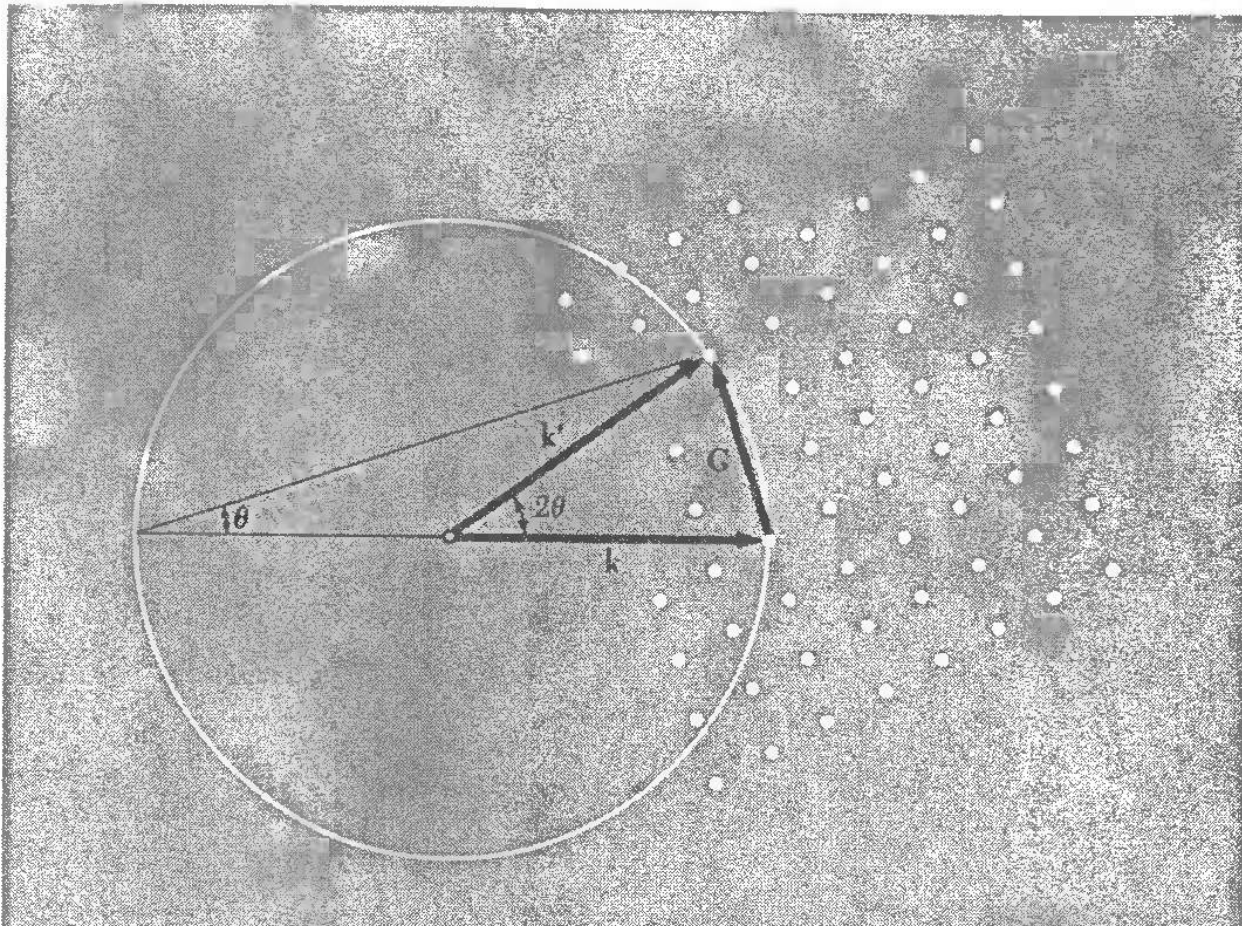
\includegraphics[width = 0.85\linewidth]{KITTEL.png}% Here is how to import EPS art
	\caption{\label{fig:KITTEL}입사, 투과벡터 관계}
\end{figure}

\subsection{\label{sec:level2}Crystal Structure of Graphite}
Graphite의 결정 구조는 Fig.\ref{fig:Graphite}와 같다.[2] 이 때 A의 탄소 원자들 사이의 결합은 강한 $\sigma$ 결합이고, 층과 층 사이의 결합은 약한 $\pi$결합이 주를 이룬다. 주어진 실험에서 사용하는 graphite는 polycrystal이므로 amplify된 scattering wave amplitude는 주로 A의 구조에서 일어난 scattering에 의한 것이다. A의 구조에서 가장 큰 간격을 가지는 cell의 구조는 빨간선의 형태로 나타날 것이다. 이 때 거리는 $d_{10} = 213pm$에 해당하며 그다음의 경우는 파란 선들에 해당하고 거리는 $d_{11} = 123pm$의 거리를 가진다.

\begin{figure}[htbp]
	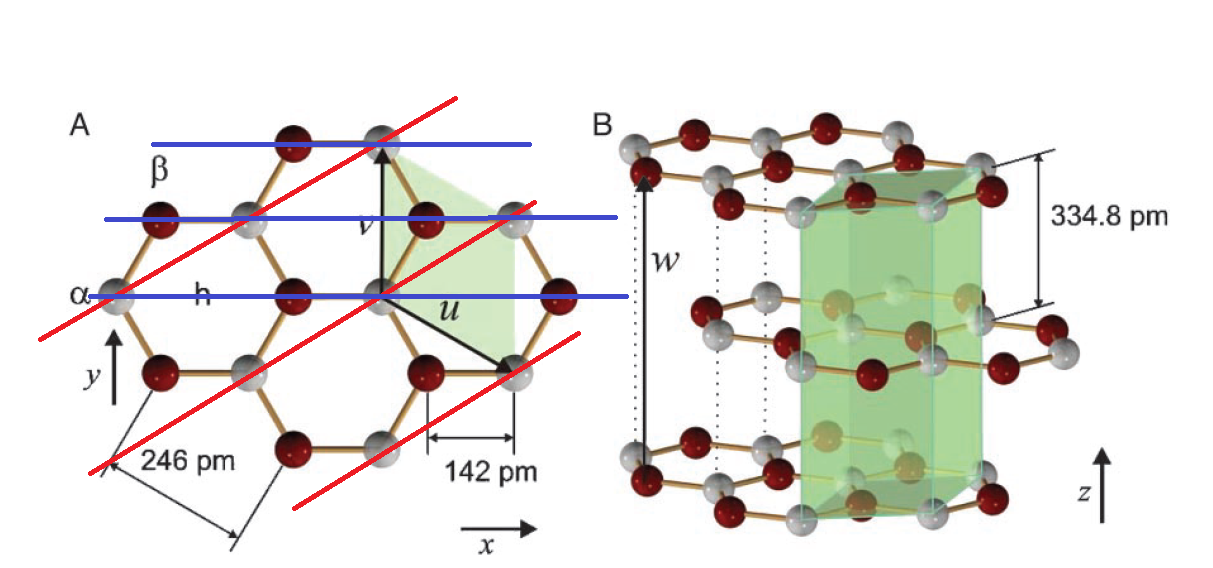
\includegraphics[width = 0.95\linewidth]{Graphite.png}% Here is how to import EPS art
	\caption{\label{fig:Graphite}Graphite의 구조}
\end{figure}

\subsection{\label{sec:level2}입자의 파동성}
입자는 입자성과 파동성을 모두 가진다. 입자의 파동성은 wave와 같이 간섭을 하는지 실험을 통해 확인하면 알 수 있다. 입자의 운동량과 파동성은 아래의 관계식을 가진다.

\begin{align}
	\lambda &= \frac{h}{p}
\end{align}

만약 입자가 $eU=p^{2}/2m$이라는 운동에너지를 가질 경우 입자의 파장은 아래와 같이 나타낼 수 있을 것이다.

\begin{align}
	\lambda &= \frac{h}{\sqrt{2meU}}
\end{align}

입자가 결정 격자를 추과하여 반지름 $R$을 가지는 원형 스크린에 원형 간섭 무늬를 만드는 조건은 식 (\ref{eq:wave_eq})에 따라 아래와 같이 쓸 수 있다. 단, 이 때 $m=1$인 경우만을 확인하며 $R_{1}$은 간섭무늬 띠의 반지름에 해당한다. 또한 아래의 식에서 $\theta$는 입사파에 대한 투과파의 각도이다.

\begin{align}
	2d(hkl) \sin \frac{\theta}{2} &= \lambda\\
	&=\frac{h}{\sqrt{2meU}}\\
	&=d(hkl)\frac{R_{1}}{\sqrt{2R^{2} + 2R\sqrt{R^{2} - R_{1}^{2}}}\cos \frac{\theta}{2}}\\
	&\simeq d(hkl)\frac{R_{1}}{\sqrt{2R^{2} + 2R\sqrt{R^{2} - R_{1}^{2}}}}
\end{align}

따라서 아래와 같이 정리된다.
\begin{align}
	\frac{1}{\sqrt{U}} &=\frac{\sqrt{2me}}{h} d(hkl)\frac{R_{1}}{\sqrt{2R^{2} + 2R\sqrt{R^{2} - R_{1}^{2}}}}
\end{align}

\section{\label{sec:level1}Experimental}
전자회절 장비에 AC전압 포트에 $6.7V$의 교류전압을 연결해 필라멘트를 가열한다. 이후에 방출되는 전자를 음극, 양극 사이에 DC전압을 인가하여 가속시킨다. 이후에 형광스크린에 나타나는 전자들의 궤적의 반지름을 측정하여 기록한다. DC전압은 $2.5kV$ 부터 $5.5kV$까지 $0.5kV$ 간격으로 증가시킨다. 

\section{\label{sec:level1}Data and Results}
첫번째, 두번째 간섭무늬 결과는 각각 Figs.\ref{fig:First}, \ref{fig:Second}와 같다. $R^{2}$값이 $1$에 매우 가까워 실험의 재현도가 매우 높다. 기울기는 $A =\frac{d\sqrt{2me}}{h} $와 같으므로 이를 통해 회절격자의 간격을 계산하면 각각 아래와 같다. 단, 오차는 선형회귀 분산을 이용해 계산하였다.

\begin{figure}[htbp]
	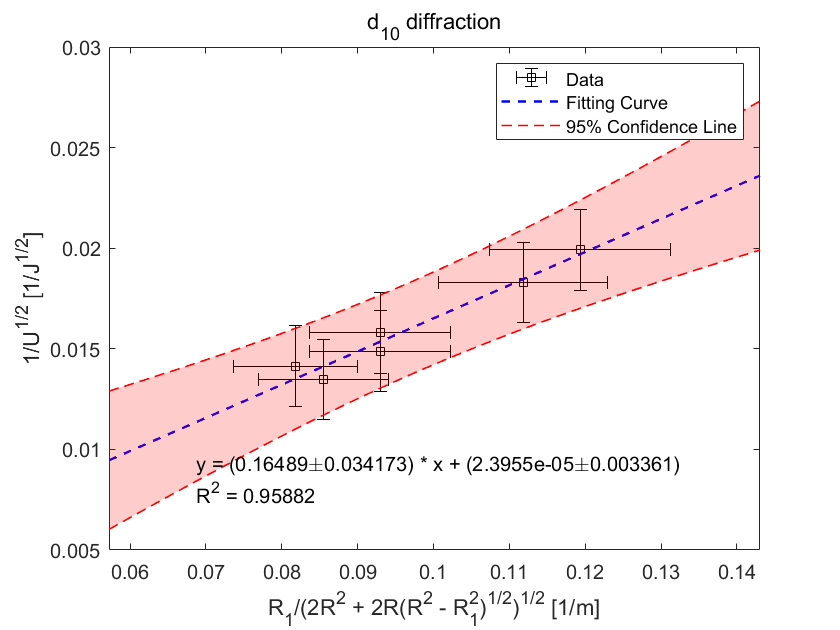
\includegraphics[width = 0.95\linewidth]{First.png}% Here is how to import EPS art
	\caption{\label{fig:First}첫번째 간섭무늬 결과}
\end{figure}

\begin{figure}[htbp]
	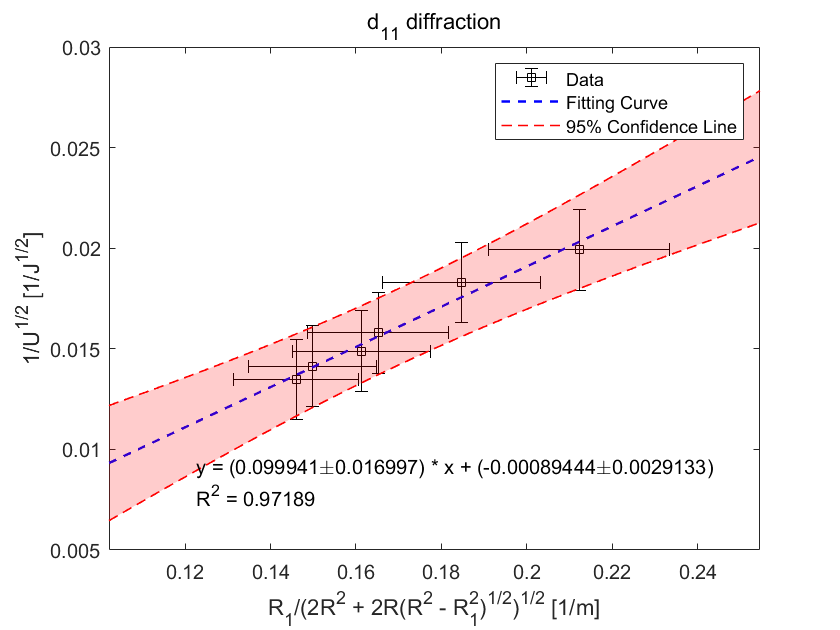
\includegraphics[width = 0.95\linewidth]{Second.png}% Here is how to import EPS art
	\caption{\label{fig:Second}두번째 간섭무늬 결과}
\end{figure}

\begin{align}
	d_{10} &= (2.02\pm0.41)\times10^{-10} [m]\\
	d_{11} &= (1.23\pm0.20)\times10^{-10} [m]
\end{align}


\section{\label{sec:level1}Discussion}
실험 결과 예측했던 격자간격값이 $10\%$이내에 존재하였다. 따라서 실험의 재현도와 정확도가 모두 높으며 이를통해 전자의 파동성이 존재함을 확인할 수 있다. 하지만 해당 실험 방식을 통해서는 $d_{12}$와 같은 격자 간격을 측정할 수 없다. 이를 해결하기 위해 충분히 높은 전압에서 실험을 수행할 수 있을 것이다. 또한 2차원 구조가 아닌 3차원 구조를 파악하기 위해서 poly crystal이 아닌 crystal을 사용하여 실험을 수행할 수 있을 것이다. 이러한 경우에는 점 격자의 형태가 실험 결과로 나타날 것이다.

\section{\label{sec:level1}Reference}
[1] C. Kittel and P. McEuen, \textit{Introduction to Solid State Physics} (Wiley, Hoboken, NJ, 2022). 

[2] S. Hembacher, F.J. Giessibl, J. Mannhart, and C.F. Quate, Proceedings of the National Academy of Sciences 100, 12539 (2003). 

\end{document}
%
% ****** End of file apssamp.tex ******
